\documentclass[12pt]{article}

\usepackage{sbc-template}
\usepackage[utf8]{inputenc}
\usepackage[brazil]{babel}
\usepackage{graphicx,url}
\usepackage{amsmath}
\usepackage{booktabs}

\sloppy

\title{Efeito Dominó no Mercado de Transferências: uma Análise Causal do Prêmio do Vendedor com Double Machine Learning}

\author{
Carlos Ferreira dos Santos Júnior\inst{1},
César de Paula Morais\inst{1},\\
Letícia Ribeiro Miranda\inst{1},
Lucas Ferreira Pedras\inst{1},\\
Lucca Alvarenga de Magalhães Pinto\inst{1}
}

\address{DCC -- Universidade Federal de Minas Gerais}

\begin{document}
\maketitle

\section{Introdução}

O mercado de transferências do futebol movimenta bilhões de euros por ano e concentra algumas das
decisões financeiras mais arriscadas da indústria esportiva. Clubes operam sob pressão de tempo,
orçamentos limitados e escrutínio público, e cada contratação equivocada tem custo esportivo e
econômico elevado. Não surpreende que a tomada de decisão no setor seja cada vez mais orientada por
dados. Um traço estrutural torna o problema particularmente difícil: o mercado funciona como uma
\textit{rede de dependências}, em que a decisão de um clube altera as condições enfrentadas pelos
demais. Compreender essas interdependências é, portanto, de interesse direto para clubes, agentes e
analistas.

Uma dessas interdependências é o que chamamos de \textit{prêmio do vendedor}. Quando um clube realiza
uma grande venda, dois sinais chegam ao mercado simultaneamente: ele passa a dispor de caixa e
adquire urgência de repor o elenco. A intuição — partilhada por dirigentes e comentaristas — é que os
vendedores percebem essa condição e cobram mais caro desse comprador nas negociações seguintes. Há,
contudo, uma armadilha analítica: clubes financeiramente robustos vendem caro \textit{e} compram caro
simultaneamente, de modo que uma correlação entre vender e pagar a mais pode refletir apenas o porte
do clube, e não um efeito causal. A pergunta de pesquisa deste trabalho é precisamente:
\textbf{a liquidez recente de um clube comprador eleva causalmente o sobrepreço que ele paga em
contratações subsequentes, uma vez neutralizados os confundidores estruturais?}

Neste trabalho, respondemos a essa pergunta com um \textit{pipeline} em duas etapas e relatamos
resultados que contrariam a intuição corrente. Primeiro, um modelo hedônico de aprendizado de máquina
estima o preço justo de cada transferência a partir de atributos do jogador, isolando como resíduo o
sobrepreço pago. Em seguida, \textit{Double Machine Learning} estima o efeito causal da liquidez do
comprador sobre esse sobrepreço, neutralizando confundidores de alta dimensão. Nossas contribuições
são três. \textbf{Primeiro}, mostramos que o efeito causal \textit{médio} é estatisticamente nulo: a
correlação positiva e significativa que aparece sem controles desaparece sob inferência causal,
revelando-se um artefato do confundidor ``clube rico''. \textbf{Segundo}, mostramos que o efeito não
é uniforme no tempo — ele emerge significativo apenas nas temporadas de 2022 e 2023, no auge da
recuperação de mercado pós-pandemia, sobrevivendo à correção de múltiplas comparações e a uma ampla
bateria de testes de robustez; o prêmio do vendedor é, assim, um fenômeno \textit{condicional ao
regime de mercado}, e não uma lei universal. \textbf{Terceiro}, propomos o \textit{Índice de
Vulnerabilidade de Barganha} como demonstração de conceito para inteligência de mercado, e
evidenciamos um alerta metodológico relevante para o setor: em análises de transferências, tratar
correlação como causa conduz a conclusões equivocadas.

Nosso trabalho diferencia-se das abordagens predominantes na literatura. Estudos que modelam o
mercado de transferências como rede concentram-se em sua \textit{estrutura} — comunidades, centralidade
e fluxos de capital — enquanto nós focamos no \textit{preço} e em sua determinação causal. Trabalhos
de avaliação de valor de jogadores, por sua vez, validam as estimativas de mercado contra desfechos
esportivos; nós as empregamos como insumo para medir desvios conjunturais de preço. A combinação de
inferência causal com aprendizado de máquina aplicada a esta pergunta é, tanto quanto sabemos, pouco
explorada. As diferenças são detalhadas na Seção~2.

O restante do artigo está organizado da seguinte forma. A Seção~2 revisa os trabalhos relacionados e
posiciona nossa contribuição. A Seção~3 descreve os dados, o pré-processamento e as duas etapas de
modelagem. A Seção~4 apresenta e discute os resultados, incluindo a comparação com a \textit{baseline}
e os testes de robustez. A Seção~5 trata das implicações práticas, e a Seção~6 conclui, apontando
limitações e direções futuras.


\section{Trabalhos Relacionados}

Este trabalho situa-se na interseção de duas literaturas: a de \textit{análise quantitativa do
mercado de transferências do futebol} e a de \textit{inferência causal com aprendizado de máquina}.
Esta seção revisa as frentes mais relevantes, destacando como cada uma fundamenta nossa metodologia
e em que pontos nossa abordagem se diferencia.

\subsection{Avaliação de valor de mercado de jogadores}

A estimativa do valor de um jogador é um problema central na economia do futebol. Uma linha
influente apoia-se na \textit{sabedoria das multidões}: as avaliações de mercado do Transfermarkt,
construídas a partir do julgamento coletivo de uma comunidade de usuários, mostram-se preditores
robustos de desfechos esportivos. Peeters \cite{peeters2018} demonstra que essas avaliações coletivas
predizem resultados de seleções nacionais com acurácia comparável ou superior à de \textit{rankings}
oficiais, evidenciando que o \textit{market value} carrega informação genuína sobre a qualidade do
atleta.

Nosso trabalho herda essa premissa, mas a aplica a uma tarefa distinta. Enquanto Peeters
\cite{peeters2018} valida o \textit{market value} contra resultados esportivos, nós o utilizamos como insumo de um
\textit{modelo hedônico} que estima o \textit{preço de transferência} (\textit{fee}) e, a partir do
resíduo desse modelo, isolamos o sobrepreço pago além do valor justo. Em vez de tomar o
\textit{market value} como verdade final, tratamo-lo como uma referência sobre a qual medimos
desvios conjunturais da negociação.

\subsection{O mercado de transferências como rede}

Uma segunda linha modela o mercado de transferências como uma \textit{rede dirigida e ponderada},
em que clubes são nós e transferências são arestas ponderadas pelo valor negociado. Esses estudos
caracterizam a estrutura do mercado — comunidades, centralidade e fluxos de capital — e relacionam a
posição estrutural de um clube ao seu desempenho.
% AMPLIAR SE HOUVER TEMPO: citar aqui \cite{wand2022,li2019,palazzo2023,dieles2023} (entradas
% comentadas em references.bib) ao descrever achados especificos da literatura de redes.

Diferentemente dessa abordagem, cujo foco está na \textit{estrutura} da rede, nosso trabalho
centra-se no \textit{preço} e no \textit{efeito causal} do histórico recente do comprador. Ainda
assim, a perspectiva de rede é incorporada de forma instrumental: métricas estruturais como
\textit{PageRank} e graus de entrada/saída entram em nosso modelo como \textit{confundidores}, para
neutralizar o fato de que clubes centrais na rede tendem a negociar valores maiores
independentemente de sua liquidez recente.

\subsection{Inferência causal com aprendizado de máquina}

Estimar um efeito causal a partir de dados observacionais exige separar a influência do tratamento
de confundidores que afetam tanto o tratamento quanto o desfecho. O arcabouço de \textit{Double/
Debiased Machine Learning} (DML) de Chernozhukov et al. \cite{chernozhukov2018} permite empregar modelos flexíveis
de aprendizado de máquina para estimar funções de confundimento de alta dimensão sem introduzir viés
de regularização no parâmetro causal, graças à ortogonalização de Neyman e ao \textit{cross-fitting}.
Adotamos esse arcabouço como núcleo da nossa estimação do efeito da liquidez sobre o sobrepreço.

Para investigar a \textit{heterogeneidade} do efeito — isto é, como ele varia entre clubes —
recorremos ao \textit{R-learner} de Nie e Wager \cite{nie2021}, que estima efeitos de tratamento
condicionais (CATE) por meio de uma formulação quasi-oráculo derivada da mesma lógica de
ortogonalização. Essa escolha nos permite construir um índice de vulnerabilidade por clube a partir
dos efeitos individuais estimados.

\subsection{Posicionamento}

Em síntese, combinamos as duas literaturas de uma forma ainda pouco explorada: aplicamos o
ferramental de inferência causal com aprendizado de máquina \cite{chernozhukov2018,nie2021} a uma
pergunta de economia do futebol tradicionalmente tratada de forma descritiva ou correlacional,
usando o \textit{market value} consagrado pela literatura \cite{peeters2018} como âncora para
definir o sobrepreço. O resultado é um desenho que distingue explicitamente o efeito causal da
liquidez do comprador do mero porte financeiro do clube — distinção que análises puramente
correlacionais ou estruturais não conseguem estabelecer.

\section{Metodologia}

Para responder se a liquidez recente de um clube comprador eleva causalmente o sobrepreço que ele
paga, adotamos um \textit{pipeline} em duas etapas encadeadas. A primeira etapa estima, por
aprendizado de máquina, o \textit{preço justo} de cada transferência a partir de atributos do
jogador, isolando como resíduo o sobrepreço pago. A segunda etapa toma esse resíduo como desfecho e
estima o efeito causal da liquidez do comprador sobre ele, neutralizando confundidores por meio de
\textit{Double Machine Learning}. Esta seção descreve os dados, o pré-processamento e as duas
etapas de modelagem.

\subsection{Conjunto de dados e pré-processamento}

Os dados foram coletados do \textit{Transfermarkt} por meio de um \textit{scraper} próprio, cobrindo
\textbf{oito temporadas} (de 2017 a 2025, com exceção de 2020, não coletada) das \textbf{sete
principais ligas europeias} (Inglaterra, Espanha, Itália, Alemanha, França, Portugal e Bélgica).
A base bruta contém \textbf{44.627 movimentações}, incluindo empréstimos, transferências gratuitas e
fins de empréstimo.

\textbf{Filtragem.} Como o objeto de estudo é o preço negociado, retemos apenas \textit{compras
pagas} com \textit{fee} e valor de mercado válidos. Transferências abaixo de \textbf{€250 mil} são
descartadas: nessa faixa o prêmio relativo é fortemente negativo e de baixa variância, indicando
ausência de dinâmica real de mercado (movimentações administrativas). Após a filtragem e a remoção
de registros incompletos, o conjunto de modelagem contém \textbf{5.146 transferências}.

\textbf{Transformações.} Os valores monetários têm forte assimetria à direita; aplicamos a
transformação logarítmica ($\log(1+x)$) ao \textit{fee} e ao valor de mercado para estabilizar a
escala. O prêmio bruto é \textit{winsorizado} nos percentis 1 e 99 para conter caudas extremas
(que chegam a milhares de pontos percentuais).

\textbf{Variáveis derivadas do clube.} Para cada clube comprador em cada temporada, agregamos a
\textit{receita de vendas} (soma dos \textit{fees} recebidos), o volume de compras (gasto total e
número de contratações) e o saldo líquido. A receita de vendas é a variável de tratamento; as
demais permitem separar o efeito de \textit{ter caixa} do comportamento habitual de gasto do clube.

\textbf{Variáveis de rede.} O mercado é modelado como um grafo dirigido e ponderado, reconstruído
por temporada, em que os nós são clubes, as arestas representam transferências (vendedor para
comprador) e o peso é o \textit{fee}. De cada clube extraímos métricas de centralidade — em
particular o \textit{PageRank} e os graus de entrada e saída — que capturam sua posição estrutural
no ecossistema e servem como controles.

\subsection{Etapa 1: modelo hedônico do preço de referência}

A primeira etapa implementa um \textit{modelo hedônico}, que decompõe o preço de um bem na soma do
valor de seus atributos. Aqui, o preço de uma transferência é explicado por características do
jogador e do contexto de mercado. A variável-alvo é o logaritmo do \textit{fee}, e o que o modelo
\textbf{não} consegue explicar — o resíduo — é interpretado como o \textit{sobrepreço de
reinvestimento}:
%
\begin{equation}
Y_{i} \;=\; \ln(P_i) \;-\; \ln(\hat{P}_i),
\label{eq:residuo}
\end{equation}
%
onde $P_i$ é o \textit{fee} pago na transferência $i$ e $\hat{P}_i$ é o preço previsto pelo modelo.
Por construção, $Y_i$ está livre das características intrínsecas do atleta; o que resta são forças
conjunturais da negociação — exatamente o objeto da Etapa 2.

\textbf{Covariáveis.} O modelo usa \textbf{19 variáveis}, todas descrevendo o jogador ou o contexto
estrutural de mercado, \textbf{nunca} o comportamento financeiro do comprador: idade e idade ao
quadrado (capturando a não-linearidade do ciclo de carreira), o logaritmo do valor de mercado,
indicadores de posição, seis \textit{dummies} de liga e sete \textit{dummies} de temporada (efeitos
fixos que absorvem a inflação de mercado). Essa separação é deliberada: reservar o comportamento
financeiro do clube para a etapa causal garante que o resíduo não o contenha de antemão.

\textbf{Modelos e avaliação.} Comparamos quatro algoritmos de regressão — \textit{Random Forest}
\cite{breiman2001}, \textit{XGBoost}, \textit{LightGBM} e \textit{Support Vector Regression} —
adotando um \textit{split} temporal: treino nas temporadas de 2017 a 2024 (4.396 observações) e
teste \textit{holdout} em 2025 (750 observações). Esse desenho simula o uso real — treinar no
passado e prever o futuro — e oferece um teste de generalização mais honesto que a partição
aleatória. A métrica principal é o RMSE, que penaliza erros grandes, relevante dada a amplitude dos
\textit{fees}. Como \textit{baseline}, avaliamos a predição usando apenas o valor de mercado, sem
aprendizado adicional. A importância das variáveis é interpretada com valores SHAP
\cite{lundberg2017}.

\textbf{Prevenção de vazamento.} O resíduo $Y_i$ que alimenta a Etapa 2 é calculado de forma
\textit{out-of-fold} (via \textit{cross-validation}): a previsão de cada observação provém de um
modelo treinado sem ela. Isso evita o vazamento que ocorreria ao usar previsões \textit{in-sample},
o qual comprimiria artificialmente a variância do resíduo e contaminaria a etapa causal.

\subsection{Etapa 2: estimação causal por Double Machine Learning}

Na segunda etapa, estimamos o efeito causal da liquidez do comprador sobre o sobrepreço. O
\textbf{tratamento} $D$ é o logaritmo da receita de vendas do clube na temporada; o \textbf{desfecho}
$Y$ é o resíduo hedônico da Etapa 1. O desafio é que diversos fatores estruturais afetam tanto a
receita quanto o sobrepreço — sobretudo o fato de que clubes grandes vendem caro \textit{e} compram
caro. Para neutralizá-los, empregamos \textit{Double/Debiased Machine Learning} (DML)
\cite{chernozhukov2018}, que assume o modelo parcialmente linear
%
\begin{equation}
Y \;=\; \theta_0\, D \;+\; g(W) \;+\; U, \qquad D \;=\; m(W) \;+\; V,
\label{eq:dml}
\end{equation}
%
em que $W$ é o vetor de confundidores e $\theta_0$ é o parâmetro causal de interesse. A ideia central
é remover de $Y$ e de $D$ a parte explicada por $W$ — usando modelos flexíveis de aprendizado de
máquina para estimar $g$ e $m$ — e estimar $\theta_0$ a partir dos resíduos ortogonalizados. Para
evitar viés de sobreajuste, as funções $g$ e $m$ são ajustadas por \textit{cross-fitting} em cinco
partições, com previsões sempre feitas fora da partição de treino. Os erros-padrão são
\textbf{clusterizados por clube e temporada}, refletindo que o tratamento varia no nível
clube-temporada.

\textbf{Confundidores.} O vetor $W$ reúne \textbf{19 variáveis}: as métricas de rede (\textit{PageRank}
e graus), o porte do elenco (tamanho, idade média, número de jogadores de seleção), além das
\textit{dummies} de liga e de temporada. Esses controles capturam o porte e a posição estrutural do
clube. Cabe registrar uma limitação: o vetor $W$ não inclui o volume financeiro \textit{direto}
(gasto total, número de compras); o confundidor de ``clube rico'' é, portanto, controlado por
\textit{proxies} estruturais, e não pelo gasto em si — ponto retomado na análise de robustez.

\textbf{Heterogeneidade e índice de vulnerabilidade.} Além do efeito médio, estimamos como o efeito
varia entre clubes. Para isso, usamos o \textit{R-learner} \cite{nie2021}, que produz um efeito
causal condicional (CATE) por observação. Agregando os efeitos por clube comprador, definimos o
\textit{Índice de Vulnerabilidade de Barganha} (IVB), que posiciona cada clube numa escala de 0 a 1:
valores altos identificam ``presas fáceis'' (clubes que pagam mais sobrepreço quando capitalizados)
e valores baixos, ``negociadores disciplinados''.

\subsection{Protocolo de validação e robustez}

Como o efeito estimado é pequeno e a identificação repousa em suposições, submetemos os resultados a
uma bateria de testes, cujos resultados são reportados na Seção~\ref{sec:resultados}. \textbf{Testes
placebo} substituem o tratamento por ruído (permutação e ruído gaussiano), verificando que o modelo
não detecta efeito espúrio. Um \textbf{teste de tratamento defasado} usa a receita da temporada
anterior — predeterminada em relação à compra atual — para avaliar causalidade reversa. Os efeitos
por temporada são submetidos a \textbf{correção de múltiplas comparações} (Bonferroni e
\textit{false discovery rate} \cite{benjamini1995}). Um \textbf{placebo de permutação intra-safra}
testa a robustez dos efeitos sazonais. Avaliamos ainda a \textbf{sensibilidade ao limiar de
\textit{fee}}, reconstruindo o \textit{pipeline} para diferentes cortes, e quantificamos a
fragilidade a confundidores omitidos pelo \textbf{\textit{Robustness Value}} \cite{cinelli2020}.
Por fim, um \textbf{teste de \textit{over-control}} reintroduz o volume financeiro no vetor de
confundidores, e \textbf{especificações alternativas do tratamento} (número de vendas e indicador de
venda de grande porte) examinam o mecanismo subjacente.

\section{Resultados e Discussão}
\label{sec:resultados}

Esta seção apresenta os resultados nas duas etapas. Primeiro, o desempenho preditivo do modelo
hedônico e sua comparação com a \textit{baseline}. Em seguida, o resultado causal central: a
correlação ingênua entre liquidez e sobrepreço desaparece sob \textit{Double Machine Learning}, mas
um efeito significativo emerge em temporadas específicas. Por fim, a heterogeneidade entre clubes e
uma bateria de testes de robustez.

\subsection{Desempenho do modelo hedônico}

A Tabela~\ref{tab:hedonico} compara os quatro modelos com a \textit{baseline}, que prevê o
\textit{fee} usando apenas o valor de mercado. Todos os modelos superam a \textit{baseline}, e o
\textit{Random Forest} obtém o melhor desempenho no \textit{holdout} de 2025, com $R^2 = 0{,}762$ e
RMSE de $0{,}673$ — um ganho de \textbf{7,4 pontos percentuais} de $R^2$ sobre a \textit{baseline}
($0{,}688$). O pequeno desvio entre validação cruzada e teste indica ausência de sobreajuste
relevante.

\begin{table}[ht]
\centering
\caption{Desempenho preditivo no \textit{holdout} de 2025 (alvo: $\log$ do \textit{fee}).}
\label{tab:hedonico}
\begin{tabular}{lcc}
\toprule
\textbf{Modelo} & \textbf{Test RMSE} & \textbf{Test $R^2$} \\
\midrule
\textit{Baseline} (só valor de mercado) & 0,769 & 0,688 \\
XGBoost                                  & 0,692 & 0,748 \\
LightGBM                                 & 0,683 & 0,754 \\
\textbf{Random Forest}                   & \textbf{0,673} & \textbf{0,762} \\
SVR (RBF)                                & 0,716 & 0,730 \\
\bottomrule
\end{tabular}
\end{table}

A análise de importância por valores SHAP \cite{lundberg2017} confirma que o valor de mercado é, de
longe, o principal preditor do \textit{fee}, seguido por idade e liga — validando empiricamente a
premissa hedônica. O resíduo resultante (o sobrepreço de reinvestimento) tem média próxima de zero
por construção, mediana de \textbf{+3,5\%} e desvio-padrão de $0{,}671$; \textbf{52,5\%} das
transferências situam-se acima do preço justo estimado. É sobre esse resíduo que a análise causal se
debruça.

\subsection{Da correlação à causa: o efeito médio}

A Figura~\ref{fig:estimadores} resume o resultado central. Uma regressão ingênua do sobrepreço
contra a liquidez, \textbf{sem controles}, estima um efeito positivo e significativo
($\theta = 0{,}0142$; IC~95\% $[0{,}0092;\,0{,}0192]$) — a evidência aparente de um ``prêmio do
vendedor''. Contudo, ao introduzir os confundidores estruturais, o efeito encolhe pela metade
($\theta = 0{,}0051$) e perde significância. Sob \textit{Double Machine Learning}
\cite{chernozhukov2018}, que controla os confundidores de forma flexível, o efeito médio é de apenas
$\theta = 0{,}0044$, com intervalo de confiança que cruza zero tanto com erros-padrão robustos
($[-0{,}0016;\,0{,}0104]$) quanto clusterizados por clube e temporada
($[-0{,}0021;\,0{,}0110]$). \textbf{O efeito causal médio é, portanto, estatisticamente nulo.}

\begin{figure}[ht]
\centering
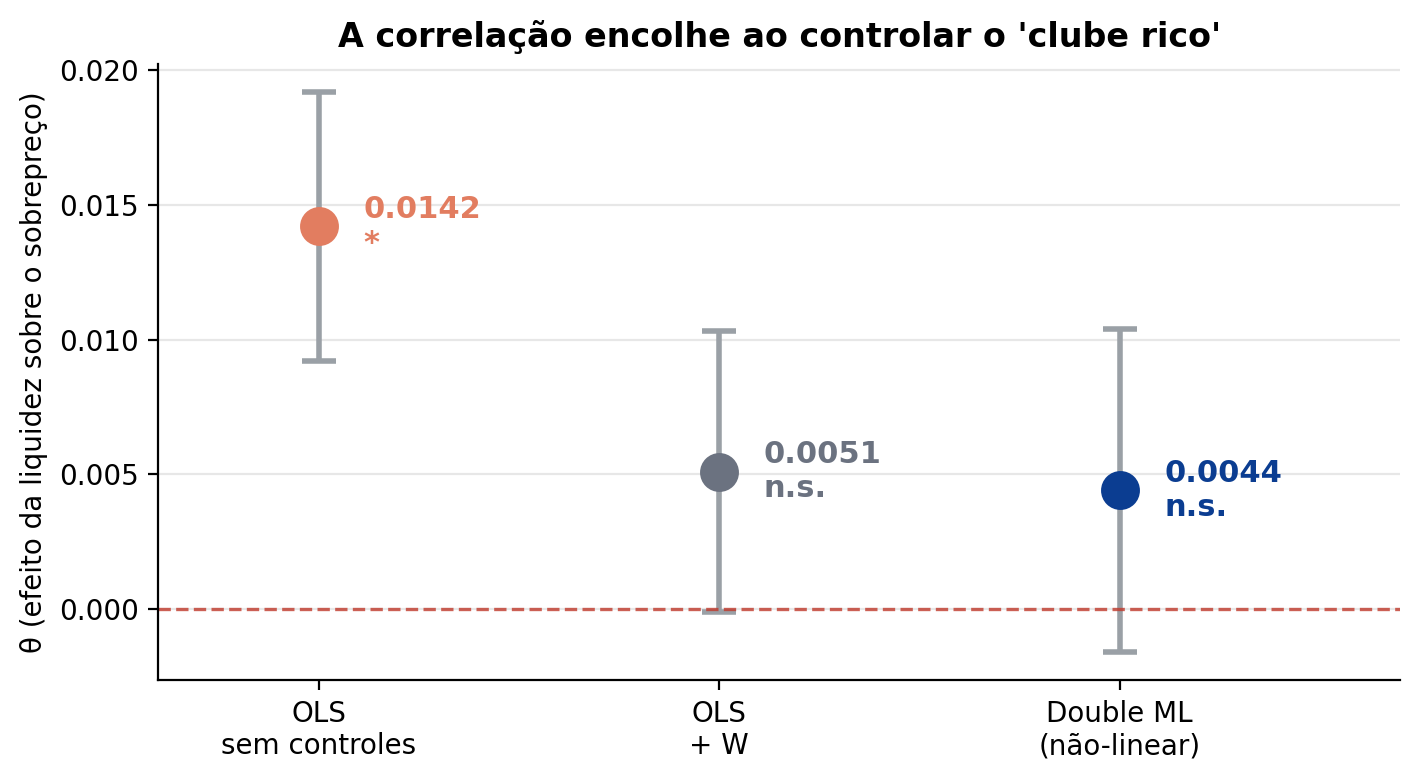
\includegraphics[width=0.7\linewidth]{imgs/comparacao_estimadores.png}
\caption{Estimativas do efeito da liquidez sobre o sobrepreço sob três especificações. A correlação
ingênua (OLS sem controles) é positiva e significativa, mas encolhe e perde significância ao
controlar os confundidores (OLS + W) e sob DML. As barras indicam o IC de 95\%.}
\label{fig:estimadores}
\end{figure}

Dois testes \textit{placebo} confirmam a validade do desenho: ao substituir o tratamento por uma
permutação aleatória ($\theta = 0{,}0024$) ou por ruído gaussiano ($\theta = 0{,}0009$), o efeito
estimado é indistinguível de zero — o modelo não detecta efeito espúrio. Note-se que o
\textit{placebo} permutado tem magnitude próxima à do efeito real, coerente com a nulidade do efeito
médio. O diagnóstico de primeira etapa mostra que os confundidores preveem moderadamente o
tratamento ($R^2 = 0{,}37$) e pouco do resíduo ($R^2 = 0{,}06$), este último esperado, já que $Y$ já
é um resíduo depurado dos atributos do jogador.

\textbf{Interpretação.} A correlação ingênua era, em grande parte, o confundidor ``clube rico'' em
ação: clubes que vendem caro também compram caro por serem financeiramente robustos, não porque a
venda os torne reféns do mercado. Sem o controle causal, concluiríamos erroneamente pela existência
de um prêmio do vendedor sistemático.

\subsection{Onde o efeito vive: heterogeneidade temporal}

A nulidade média, porém, esconde forte heterogeneidade no tempo. A Figura~\ref{fig:sazonal} mostra o
efeito estimado por temporada. De 2017 a 2021 e em 2024--2025, o efeito é indistinguível de zero.
Em \textbf{2022} ($\theta = 0{,}064$; $p = 0{,}0006$) e \textbf{2023} ($\theta = 0{,}047$;
$p = 0{,}0024$), contudo, o prêmio do vendedor é positivo e significativo — e, crucialmente,
\textbf{ambos sobrevivem à correção de Bonferroni e ao controle de \textit{false discovery rate}}
\cite{benjamini1995} para os oito testes sazonais, afastando a hipótese de falso-positivo por
testagem múltipla.

\begin{figure}[ht]
\centering
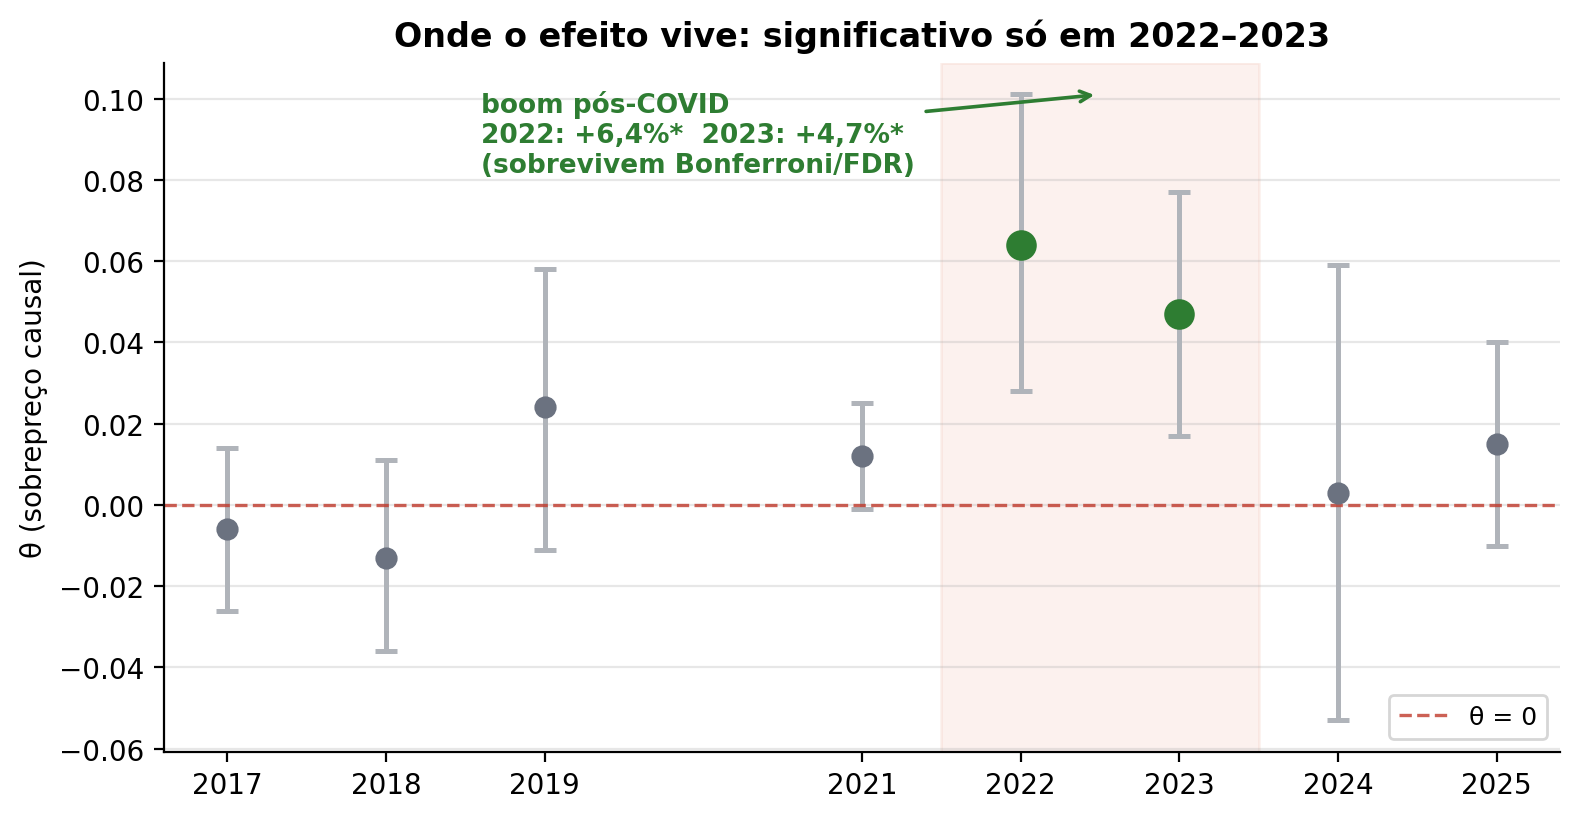
\includegraphics[width=0.8\linewidth]{imgs/theta_sazonal.png}
\caption{Efeito causal da liquidez sobre o sobrepreço, estimado por temporada (IC de 95\%
clusterizado). O efeito é nulo na maioria dos anos e significativo apenas em 2022 e 2023, no auge da
recuperação de mercado pós-pandemia.}
\label{fig:sazonal}
\end{figure}

Esses são justamente os anos do \textbf{boom de mercado pós-COVID}, quando o volume de transferências
atingiu níveis recordes após duas temporadas de retração. Nesse regime de mercado aquecido — com
escassez de alvos disponíveis e urgência de reposição — clubes capitalizados de fato pagam mais. O
achado central deste trabalho é, portanto, que \textbf{o prêmio do vendedor não é uma lei universal
do mercado, mas um fenômeno condicional ao regime}. Análises de janelas curtas (como a de três
temporadas usada em iterações anteriores deste projeto) podem capturar espuriamente um efeito médio
significativo ao concentrarem-se em anos atípicos.

\subsection{Heterogeneidade entre clubes: o IVB}

Estendendo a análise ao nível de clube, o \textit{R-learner} \cite{nie2021} estima um efeito
condicional por transferência, agregado por clube comprador no \textit{Índice de Vulnerabilidade de
Barganha} (IVB). Conceitualmente, o IVB ordena clubes entre ``presas fáceis'' (que pagam mais
sobrepreço quando capitalizados) e ``negociadores disciplinados''. \textbf{Este resultado deve ser
lido com cautela}: os efeitos condicionais têm baixo poder estatístico ($R^2$ de primeira etapa do
desfecho de apenas $0{,}06$) e o ordenamento é sensível a clubes com poucas transações, sendo o topo
do \textit{ranking} dominado por um \textit{outlier}. Tratamos o IVB, portanto, como uma
\textbf{demonstração de conceito exploratória} — uma direção promissora para inteligência de
mercado (Seção~\ref{sec:aplicacoes}), não como um resultado conclusivo.

\subsection{Robustez}

Submetemos o achado a uma bateria de testes, sintetizada na Tabela~\ref{tab:robustez}. O efeito
sazonal de 2022--2023 mostra-se robusto: um \textit{placebo} de permutação intra-safra produz
$p$ empírico de $0{,}005$; o efeito é estável a variações do limiar de \textit{fee} (de €0 a €1M); e
o \textit{Robustness Value} \cite{cinelli2020} de $\approx 0{,}24$--$0{,}27$ indica que um
confundidor omitido precisaria explicar cerca de um quarto da variação residual do tratamento
\textit{e} do desfecho para anular o efeito. Mesmo num teste de \textit{over-control}, que
reintroduz o volume financeiro no vetor de confundidores, o efeito de 2023 sobrevive
($p \approx 0{,}003$), embora o de 2022 atenue.

Dois resultados qualificam a interpretação. O \textbf{teste de tratamento defasado} (liquidez da
temporada anterior) é significativo ($\theta = 0{,}0051$), o que enfraquece a hipótese de
causalidade reversa; porém, como o efeito contemporâneo na mesma subamostra é não significativo, o
teste \textbf{não é conclusivo}. Especificações alternativas do tratamento — número de vendas e
indicador de venda de grande porte — são significativas isoladamente ($\theta = 0{,}049$ e
$0{,}075$), sugerindo um mecanismo de ``sinalização de necessidade''; entretanto, ao controlar a
intensidade de atividade do clube, ambas perdem significância, de modo que esse mecanismo permanece
como \textbf{hipótese exploratória}, não como achado confirmado.

\begin{table}[ht]
\centering
\caption{Síntese da bateria de robustez.}
\label{tab:robustez}
\begin{tabular}{lll}
\toprule
\textbf{Teste} & \textbf{Resultado} & \textbf{Leitura} \\
\midrule
\textit{Placebo} (permutação / ruído)      & $\theta \approx 0{,}002$ / $0{,}001$ & desenho não gera efeito espúrio \\
Bonferroni / FDR (8 testes sazonais)        & 2022 e 2023 sobrevivem & efeito sazonal não é falso-positivo \\
\textit{Placebo} permutação intra-safra     & $p_{emp} = 0{,}005$ & efeito de 2022--2023 é real \\
Sensibilidade ao limiar de \textit{fee}     & estável (€0--€1M) & não é artefato do corte \\
\textit{Robustness Value}                   & $0{,}24$--$0{,}27$ & confundidor omitido teria de ser forte \\
\textit{Over-control} (com volume financeiro)& 2023 sobrevive ($p\approx0{,}003$) & robusto a controle financeiro direto \\
Tratamento defasado (C2)                     & $\theta = 0{,}0051$ (não conclusivo) & causalidade reversa enfraquecida \\
Tratamentos alternativos (vendas / porte)    & signif.\ isolado, n.s.\ com controle & mecanismo exploratório \\
\bottomrule
\end{tabular}
\end{table}

\section{Aplicações e Implicações Práticas}
\label{sec:aplicacoes}

Os resultados têm implicações diretas para clubes, agentes e analistas de mercado. Discutimos três:
o \textit{timing} de contratações, a inteligência de mercado baseada em vulnerabilidade de barganha
e um alerta metodológico para a análise de transferências.

\textbf{\textit{Timing} de contratações.} O achado de que o prêmio do vendedor é condicional ao
regime de mercado tem valor operacional. Em janelas de mercado aquecido — como 2022 e 2023 — a
liquidez recente elevou significativamente o sobrepreço pago, com efeito causal estimado entre
\textbf{4,7\% e 6,4\%} (por unidade logarítmica de receita de vendas); fora desses anos, o efeito é
estatisticamente nulo. Para um clube com poder de espera, isso sugere uma vantagem estrutural: adiar a
reposição para fora do pico de mercado, ou desacoplar a decisão de compra da entrada de caixa de uma
venda, pode evitar um sobrepreço material. Para um clube vendedor, o mesmo padrão indica o momento
oportuno para negociar com compradores pressionados. Fora desses regimes, contudo, não há evidência
de que reter ou acelerar a compra altere sistematicamente o preço — uma conclusão igualmente útil,
pois desencoraja heurísticas de negociação infundadas.

\textbf{Inteligência de mercado e o IVB.} O \textit{Índice de Vulnerabilidade de Barganha}, ainda que
exploratório nesta versão, ilustra um produto analítico concreto: um \textit{ranking} de clubes por
propensão a pagar sobrepreço sob liquidez. Operacionalizado com dados mais ricos e estimadores mais
robustos, o IVB poderia integrar ferramentas de \textit{scouting} financeiro — sinalizando, do lado
comprador, clubes que precisam de disciplina de negociação, e, do lado vendedor, alvos comerciais
mais permeáveis a prêmios. A contribuição aqui é metodológica: mostramos como efeitos causais
heterogêneos podem ser convertidos num índice acionável por clube.

\textbf{Alerta metodológico.} Talvez a implicação mais ampla seja de método. Uma análise puramente
correlacional do mesmo conjunto de dados concluiria pela existência de um prêmio do vendedor
sistemático e significativo ($\theta = 0{,}0142$). Foi apenas ao isolar o efeito causal, controlando
o porte e a posição estrutural dos clubes, que essa conclusão se revelou um artefato do confundidor
``clube rico''. Em um setor que investe cada vez mais em análise de dados, o caso é um lembrete
prático de que \textbf{correlação não é causalidade}: decisões de mercado de alto valor — orçamentos,
estratégias de contratação, avaliação de janelas — exigem desenhos que separem efeito de seleção.
O ferramental de inferência causal com aprendizado de máquina empregado aqui oferece um caminho
viável para essa distinção em dados observacionais de mercado.


\section{Conclusão e Trabalhos Futuros}

Este trabalho investigou se a liquidez recente de um clube comprador — o caixa gerado por vendas —
eleva causalmente o sobrepreço que ele paga em contratações subsequentes, o chamado ``prêmio do
vendedor''. Para isso, propusemos um \textit{pipeline} em duas etapas: um modelo hedônico que isola
o sobrepreço como resíduo do preço justo, e uma estimação de \textit{Double Machine Learning} que
mede o efeito causal da liquidez sobre esse resíduo, neutralizando confundidores estruturais.

\textbf{Principais descobertas.} O modelo hedônico alcançou $R^2$ de $0{,}762$ no \textit{holdout},
superando em 7,4 pontos a \textit{baseline} de valor de mercado. Na etapa causal, o achado central é
duplo. Primeiro, o \textbf{efeito médio é estatisticamente nulo}: a correlação positiva e
significativa que aparece sem controles ($\theta = 0{,}0142$) desaparece sob DML
($\theta = 0{,}0044$, com intervalo cruzando zero), revelando-se um artefato do confundidor ``clube
rico''. Segundo, e mais importante, o efeito \textbf{não é uniforme no tempo}: emerge significativo
apenas em 2022 e 2023 — o auge da recuperação de mercado pós-pandemia — sobrevivendo à correção de
múltiplas comparações e a uma bateria de testes de robustez. O prêmio do vendedor, portanto, não é
uma lei universal do mercado, mas um \textbf{fenômeno condicional ao regime}.

\textbf{Contribuições.} Destacamos: (i) a aplicação de inferência causal com aprendizado de máquina
a uma questão de economia do futebol tradicionalmente tratada de forma correlacional; (ii) a
evidência de que o prêmio do vendedor é condicional ao aquecimento do mercado, o que reconcilia
resultados aparentemente positivos de janelas curtas com a nulidade de longo prazo; (iii) o
\textit{Índice de Vulnerabilidade de Barganha} como demonstração de conceito para inteligência de
mercado; e (iv) um alerta metodológico sobre os riscos de interpretar correlação como causa na
análise de transferências.

\textbf{Limitações.} A principal restrição é a \textbf{granularidade temporal}: o tratamento é
medido por temporada, e não pela janela de poucos dias em que o ``efeito dominó'' originalmente se
manifestaria — o que dilui o efeito e torna nossas estimativas conservadoras. Além disso, o controle
do confundidor ``clube rico'' apoia-se em \textit{proxies} estruturais (rede, elenco, liga), e não no
volume financeiro direto; o confundidor de causa comum (reestruturação estratégica) não é tratado; o
modelo hedônico não incorpora desempenho individual do atleta, de modo que parte do valor esportivo
pode vazar para o resíduo; e a estimativa de heterogeneidade que sustenta o IVB tem baixo poder,
tornando o índice ilustrativo.

\textbf{Trabalhos futuros.} Várias direções decorrem dessas limitações. A obtenção de \textbf{datas
exatas} das transações permitiria estimar a curva de decaimento temporal do efeito e endereçar
diretamente a causalidade reversa. A \textbf{integração de métricas de desempenho} (gols,
assistências, \textit{expected goals}) refinaria o preço justo e depuraria o resíduo. Do lado
causal, o uso de \textbf{\textit{Propensity Score Matching}} como validação complementar e de
\textit{Causal Forests} para uma estimativa de heterogeneidade mais robusta consolidaria o IVB.
Por fim, uma análise simétrica do \textbf{lado vendedor} identificaria ``clubes predadores'' — os que
extraem prêmios de forma sistemática — fechando o quadro do ecossistema de transferências.


\bibliographystyle{sbc}
\bibliography{sbc}

\end{document}
